%!TEX root = ../thesis.tex
%*******************************************************************************
%*********************************** Seventh Chapter *****************************
%*******************************************************************************

\chapter{Centre Vortex Visualisations}\label{chapter:Visualisations}
\ifpdf
    \graphicspath{{Chapter7/Figs/Raster/}{Chapter7/Figs/PDF/}{Chapter7/Figs/}}
\else
    \graphicspath{{Chapter7/Figs/Vector/}{Chapter7/Figs/}}
\fi

In previous chapters we have motivated the significance of centre vortices in QCD through the calculation of the gluon propagator. Although we can predict many of the properties of vortices through calculation, these properties can also be explored through visualisations of the lattice. To this end, in this chapter we present a novel visualisation technique that allows us to view thin centre vortices on the lattice through the use of 3D models~\footnote{All 3D models have been generated using Advanced Visual Systems (AVS) Express Visualisation Edition, version 8.4.1.}. These models allow for a highly interactive exploration of the vortex structure of the QCD vacuum.

\section{Space-Oriented Vortices}
As the lattice is a four-dimensional hypercube, we visualise the centre vortices on a set of 3D slices. The choice of dimension to take slices along is irrelevant in Euclidean space, so we choose to take slices along the $x$-axis, resulting in $N_x$ slices each with dimensions $N_y\times N_z\times N_t$. This choice of axis to slice along allows for the largest volume per slice.  However, the transition between slices is most intuitively thought of as `stepping though time', so we re-label our coordinates such that each slice is considered to be a snapshot at fixed $t$, with local coordinates $(x,y,z)$. Within each slice we can visualise all vortices associated with an $x-y$, $x-z$ or $y-z$ plaquette by calculating $P_{x\,y}(\bf{x})$, $P_{y,z}(\bf{x})$ and $P_{z,x}(\bf{x})$ for all $\bf{x}$ in the slice. These vortices will be referred to as the `space-oriented' vortices, as they are fixed in time. The plaquettes are evaluated on a centre projected configuration, so $P_{\mu\nu}\in \lbrace -1,\,0,\,+1\rbrace$. For a $+1$ vortex, a blue jet is plotted piercing the centre of the plaquette, and for a $-1$ vortex a red jet is plotted. The direction of the jet is set according to a right-hand rule, such that
\begin{itemize}[leftmargin=*,itemsep=0pt,labelsep=12pt]
\item $P_{x\,y}=\pm 1\implies \pm\hat{z}$ direction.
\item $P_{y\,z}=\pm 1\implies \pm\hat{x}$ direction.
\item $P_{x\,z}=\pm 1\implies \mp\hat{y}$ direction,
\end{itemize}
An example of this plotting convention is shown in Fig.~\ref{fig:SpacialVortices}.\\

\begin{figure}[ht]
\centering
  \begin{subfigure}[b]{0.3\textwidth}
  \centering
  \begin{tikzpicture}[scale=0.9]
\begin{scope}[very thick,decoration={
    markings,
    mark=at position 0.5 with {\arrow[scale=2]{stealth}}}
    ] 
  % bottom right to top right                    x,y start of line    label  x,y end
  \draw[line width=1.0,postaction={decorate}](1.5,-1.5)-- node[left]{$Z_y(x+\hat x)\ $} (3.25,1.5)node(g){};
  % top right to top left
  \draw[line width=1.0,postaction={decorate}](3.25,1.5)-- node[above]{${}\ \ Z_x^*(x+\hat y)$} (-1.5,1.5);
  % top left to bottom left
  \draw[line width=1.0,postaction={decorate}](-1.5,1.5)-- node[left]{$Z_y^*(x)$}(-4,-1.5);

  % Jet triangle
  % bottom left	
  \draw (-0.3,-2) node(a){}
  -- (0.1,-2) node(b){}   % bottom right
  -- (-0.1,2) node(c){}   % top
  -- cycle;               % complete
  \fill[blue] (a.center) -- (b.center) -- (c.center);
  
  % bottom left to bottom right
  \draw[line width=1.0,postaction={decorate}](-4,-1.5)-- node[above]{$Z_x(x)$}(1.5,-1.5)node(f){};
  
  \draw[line width=1.0,-{Latex[length=2mm]}](-5,0)--(-4,0.0)node[right]{\large $x$};
  \draw[line width=1.0,-{Latex[length=2mm]}](-5,0)--(-4.6,0.8)node[right]{\large $y$};
  \draw[line width=1.0,-{Latex[length=2mm]}](-5,0)--(-5,1.0)node[above]{\large $z$};
  \end{scope}
  
\end{tikzpicture}
  \end{subfigure}
  \hfill
  \begin{subfigure}[b]{0.55\textwidth}
  \centering
  \begin{tikzpicture}[scale=0.9]
\begin{scope}[very thick,decoration={
    markings,
    mark=at position 0.5 with {\arrow[scale=2]{stealth}}}
    ] 
  % bottom right to top right                    x,y start of line    label  x,y end
  \draw[line width=1.0,postaction={decorate}](1.5,-1.5)-- node[left]{$Z_y(x+\hat x)\ $} (3.25,1.5)node(g){};
  % top right to top left
  \draw[line width=1.0,postaction={decorate}](3.25,1.5)-- node[above]{\quad $Z_x^*(x+\hat y)$} (-1.5,1.5);
  % top left to bottom left
  \draw[line width=1.0,postaction={decorate}](-1.5,1.5)-- node[left]{$Z_y^*(x)$}(-4,-1.5);

  % Jet triangle
  \draw (-0.3,2) node(a){}
  -- (0.1,2) node(b){}
  -- (-0.1,-2)node(c){}
  -- cycle;
  \fill[red] (a.center) -- (b.center) -- (c.center);
  
  % bottom left to bottom right
  \draw[line width=1.0,postaction={decorate}](-4,-1.5)-- node[above]{$Z_x(x)$}(1.5,-1.5)node(f){};
  
  % Coordinate axes       arrow head          x,y start -- x,y finish [position] label
  \end{scope}
\end{tikzpicture}
  \end{subfigure}             
  \caption{An example of the plotting convention for vortices located within a 3D time slice. \textbf{Left:} A $+1$ vortex in the $+\hat{z}$ direction. \textbf{Right:} A $-1$ vortex in the $-\hat{z}$ direction.}
  \label{fig:SpacialVortices}
\end{figure}
%
The 3D slices for $t=1,2$ with the space-oriented vortices plotted appear as in Figs.~\ref{fig:PlaqT01}, \ref{fig:PlaqT02}. At first glance the vortex structure appears highly complex, and it is difficult to identify the significant features. As such, we make use of the 3D models to hone in and isolate the important features present in these slices. We present some of these features in Fig.~\ref{fig:VortexFeatures}.\\

%
{\centering
\begin{figure}
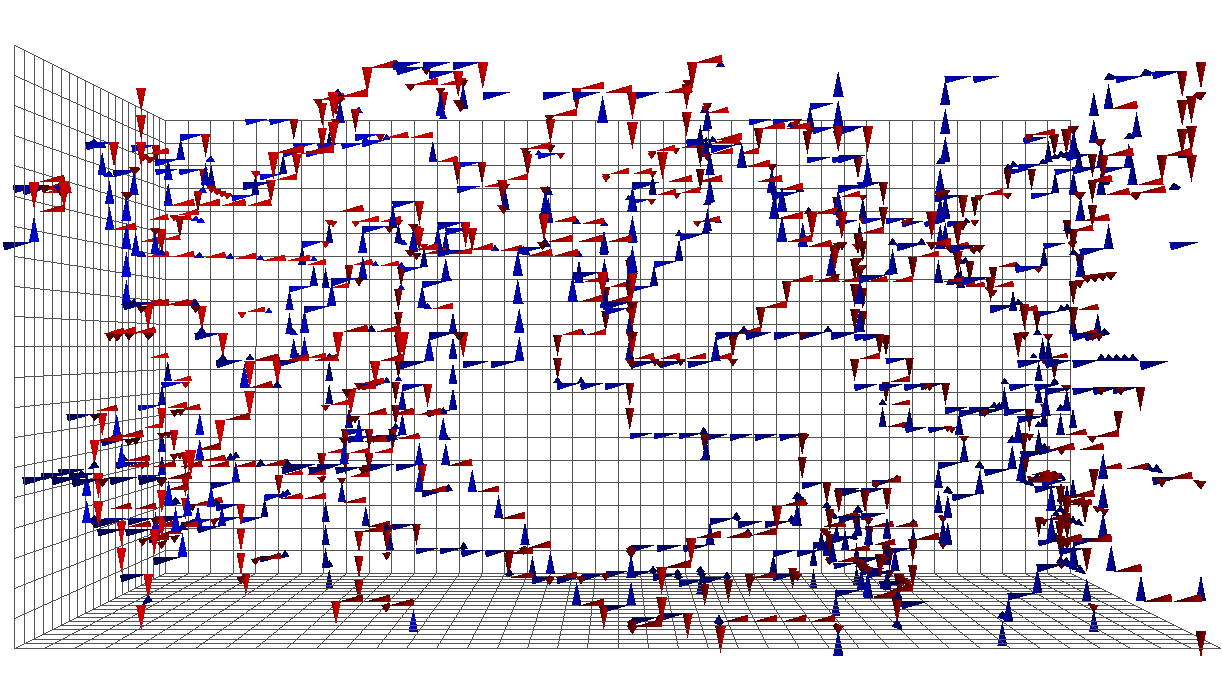
\includegraphics[width=\linewidth]{Plaq_CFG95_T01.png}
\caption{\label{fig:PlaqT01}The $t=1$ slice with all space-oriented vortices plotted.}
\end{figure}
}
%
{\centering
\begin{figure}
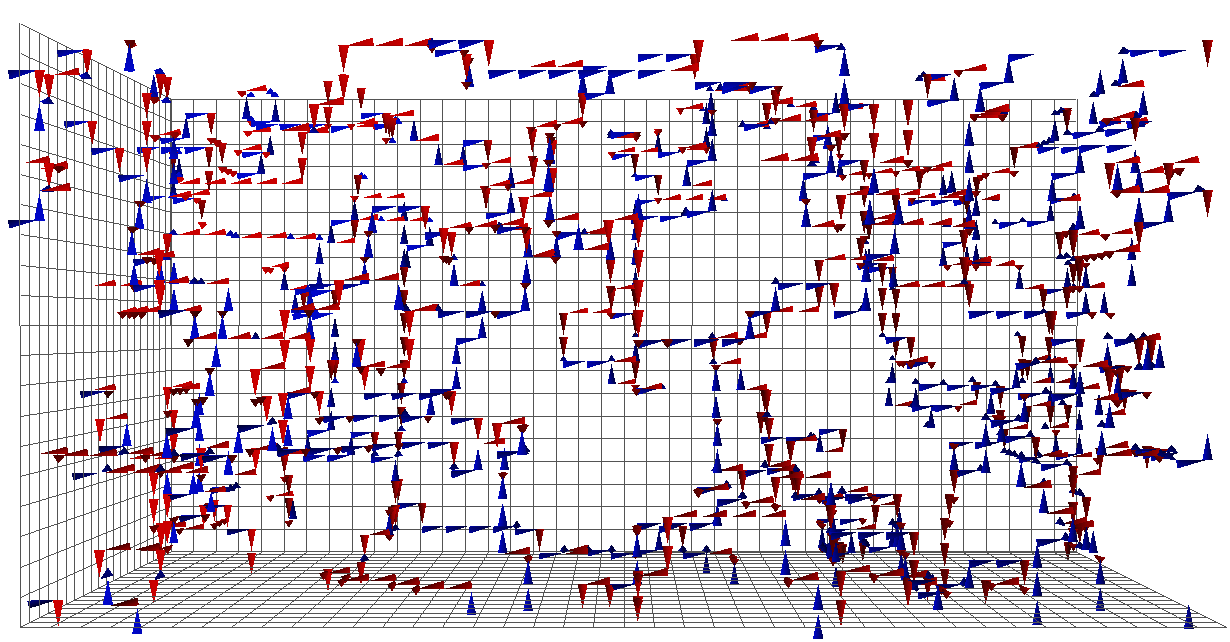
\includegraphics[width=\linewidth]{Plaq_CFG95_T02.png}
\caption{\label{fig:PlaqT02}The $t=2$ slice with all space-oriented vortices plotted.}
\end{figure}
}
%
\begin{figure}[htb!]
\centering
    \begin{subfigure}[b]{0.3\textwidth}
	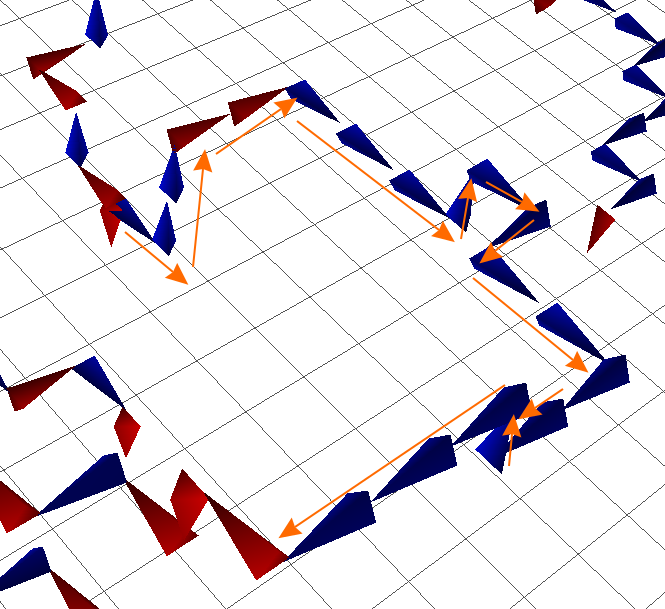
\includegraphics[width=\textwidth]{./plaqt1_line.png}
    \end{subfigure}\hfill
    \begin{subfigure}[b]{0.3\textwidth}
    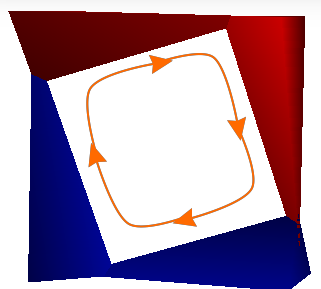
\includegraphics[width=\textwidth]{./plaqt1_loop.png}
    \end{subfigure}\hfill
    \begin{subfigure}[b]{0.3\textwidth}
	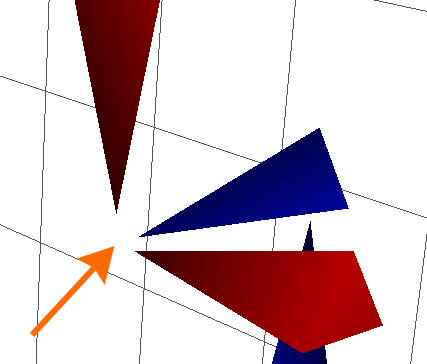
\includegraphics[width=\textwidth]{./plaqt1_monopole.png}
    \end{subfigure}
    \caption{\label{fig:VortexFeatures} \textbf{Left:} Vortices form continuous lines. Note that because of the lattice periodicity, these lines may wrap around to the opposite edge of the lattice. \textbf{Middle:} Vortices must form closed loops to conserve the vortex flux. \textbf{Right:} $SU(3)$ vortices are capable of forming monopoles or branching points where three vortices emerge or converge at a single point.}
\end{figure}
%
It is an excellent sanity check to see that the vortices do indeed form closed lines, as they must to conserve the centre flux and satisfy the Bianchi identity~\cite{Engelhardt:2003wm,Spengler:2018dxt}. We also observe that with the exception of the $1\times 1$ vortex loops (see the middle image in Fig.~\ref{fig:VortexFeatures}) which can be readily attributed to incorrectly identified centre phases, the vortex loops are large and rarely form isolated loops within the 3D volume. This agrees with the observation made of $SU(2)$ vortices in Refs.~\cite{Engelhardt:1999fd,Bertle:1999tw} that below the critical deconfinement temperature, $T_C$, almost all vortices identified had the maximum possible extent. It will be the subject of future work to investigate whether as the temperature increases the $SU(3)$ vortices begin to shrink and cease to percolate, indicating a transition to the deconfining phase.\\

The presence of branching/monopole points is of particular interest, as previous studies have primarily focussed on $SU(2)$ theory which is free from these structures. This is because it is only in $SU(3)$ (or more generally, $SU(N)$ with $N>2$) that it is possible to conserve the centre flux at the intersection of 3 vortices, as shown in Fig.~\ref{fig:VortexBranching}. It is clear from our visualisations that these points occur frequently in the confining phase, in agreement with the findings of Ref.~\cite{Spengler:2018dxt}. The ambiguity between monopoles and branching points arises from the lack of definite orientation for the vortex line. As $P_{\nu\mu} = P_{\mu\nu}^\dagger$, the ordering by which the plaquette is calculated will invert the sign of the vortex, and as such the choice of ordering can change a monopole into a branching point, or vice-versa. The lack of definite orientation for vortices is an important property, as it permits non-vanishing topological charge, and is indeed a key property of the vortex model~\cite{Engelhardt:2010ft,Engelhardt:1999xw}. The presence of these points may also enforce an integer topological charge when they are considered to be `nexus' solutions, as described in Refs.~\cite{Cornwall:1999xw,Cornwall:1998ef}.
%
\begin{figure}[htb!]
\centering
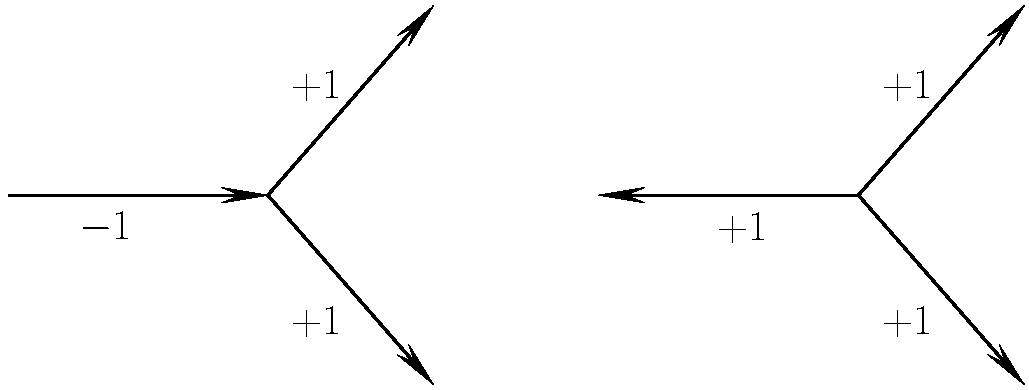
\includegraphics[width=\linewidth]{./VortexBranching.pdf}
\caption{\label{fig:VortexBranching}\textbf{Left:} A vortex branching point. \textbf{Right:} A vortex monopole. Note that for both figures, the vortex charge is conserved at the vertex. By changing the orientation of the plaquette containing the left-most vortex, these two diagrams can be interchanged.}
\end{figure}
%
\section{Time-Oriented Vortices}
For each link in a given 3D slice there are two additional plaquettes that lie in the $x_i - t$ plane, pointing in the positive and negative time directions. Vortices associated with time-oriented plaquettes contain information of how the line-like vortices evolve with time, or equivalently, how the vortex surfaces appear in four dimensions. In a given 3D slice we only have access to one link associated with a time-oriented vortex, and as such we plot an arrow along this link to indicate its association with this vortex. We adopt the following plotting convention for these time-oriented vortices:
\begin{itemize}[leftmargin=*,itemsep=0pt,labelsep=12pt]
\item  \makebox[13em][l]{$+1$ vortex, forward in time}  $\implies$ cyan arrow, positively oriented.
\item  \makebox[13em][l]{$+1$ vortex, backward in time} $\implies$ cyan arrow, negatively oriented.
\item  \makebox[13em][l]{$-1$ vortex, forward in time}  $\implies$ orange arrow, positively oriented.
\item  \makebox[13em][l]{$-1$ vortex, backward in time} $\implies$ orange arrow, negatively oriented.
\end{itemize}
An example of these conventions is shown in Fig.~\ref{fig:TimeVortices}. Utilising these conventions, we see that the first two time slices now appear as Figs.~[\ref{fig:PlaqLinkT01}, \ref{fig:PlaqLinkT02}]\\
%
\begin{figure}[ht]
\centering
  \begin{subfigure}[b]{0.45\textwidth}
  \centering
  \begin{tikzpicture}[scale=0.7]
% Axes
\tkzDefPoint(-6,-1.5){ax}
\tkzDefShiftPoint[ax](1,0){axR}
\tkzDefShiftPoint[ax](0,1){axT}
\tkzDefShiftPoint[ax](0.6,0.8){axB}

\begin{scope}[very thick,decoration={
    markings,
    mark=at position 0.5 with {\arrow[scale=2]{stealth}}}
    ] 

  % cyan line first to make it look transparent
  \draw[line width=5,color=cyan,-{Latex[length=6mm]}](-4.0,-1.5)--(1.5,-1.5);

  % bottom right to top right                    x,y start of line    label  x,y end
  \draw[line width=1.0,postaction={decorate}](1.5,-1.5)--node[right]{} (3.25,1.5)node(g){};
  % top right to top left
  \draw[line width=1.0,postaction={decorate}](3.25,1.5)--node[above]{} (-1.5,1.5);
  % top left to bottom left
  \draw[line width=1.0,postaction={decorate}](-1.5,1.5)--node[left]{} (-4,-1.5);

  \filldraw[fill=blue,fill opacity=0.2] (-4,-1.5) -- (1.5,-1.5) -- (1.5,4) -- (-4,4)--cycle;

  %% % Jet triangle
  %% % bottom left	
  %% \draw (-0.3,-2) node(a){}
  %% -- (0.1,-2) node(b){}   % bottom right
  %% -- (-0.1,2) node(c){}   % top
  %% -- cycle;               % complete
  %% \fill[red] (a.center) -- (b.center) -- (c.center);
  
  % bottom left to bottom right
  \draw[line width=1.0,postaction={decorate}](-4.0,-1.5)--node[above]{}(1.5,-1.5)node(f){};
  
  % t direction  
  \draw[line width=1.0,postaction={decorate}]( 1.5,-1.5)--node[right]{} (1.5,4.0);    % width  3.25-(-1.5) = 4.75
  \draw[line width=1.0,postaction={decorate}]( 1.5, 4.0)--node[above]{}(-4.0,4.0);    % height 6.25-1.5    = 4.75
  \draw[line width=1.0,postaction={decorate}](-4.0, 4.0)--node[left]{}(-4.0,-1.5);

  \end{scope}
  
% Draw Axes
\tkzDrawSegments[thick,->, >=stealth](ax,axR)
\tkzDrawSegments[thick,->, >=stealth](ax,axT)
\tkzDrawSegments[thick,->, >=stealth](ax,axB)
\tkzLabelPoint[right](axR){$x$}
\tkzLabelPoint[above](axT){$t$}
\tkzLabelPoint[above](axB){$y$}
\end{tikzpicture}
  \end{subfigure}
  \hfill
  \begin{subfigure}[b]{0.45\textwidth}
  \centering
  \begin{tikzpicture}[scale=0.7]
\begin{scope}[very thick,decoration={
    markings,
    mark=at position 0.5 with {\arrow[scale=2]{stealth}}}
    ] 

  % orange line first to make it look transparent
  \draw[line width=5,color=orange,-{Latex[length=6mm]}](-4.0,-1.5)--(1.5,-1.5);

  % bottom right to top right                    x,y start of line    label  x,y end
  \draw[line width=1.0,postaction={decorate}](1.5,-1.5)--node[right]{} (3.25,1.5)node(g){};
  % top right to top left
  \draw[line width=1.0,postaction={decorate}](3.25,1.5)--node[above]{} (-1.5,1.5);
  % top left to bottom left
  \draw[line width=1.0,postaction={decorate}](-1.5,1.5)--node[left]{} (-4,-1.5);

    \filldraw[fill=red,fill opacity=0.2] (-4,-1.5) -- (1.5,-1.5) -- (1.5,4) -- (-4,4)--cycle;
  
  %% % Jet triangle
  %% % bottom left	
  %% \draw (-0.3,-2) node(a){}
  %% -- (0.1,-2) node(b){}   % bottom right
  %% -- (-0.1,2) node(c){}   % top
  %% -- cycle;               % complete
  %% \fill[red] (a.center) -- (b.center) -- (c.center);
  
  % bottom left to bottom right
  \draw[line width=1.0,postaction={decorate}](-4.0,-1.5)--node[above]{}(1.5,-1.5)node(f){};
  
  % t direction  
  \draw[line width=1.0,postaction={decorate}]( 1.5,-1.5)--node[right]{} (1.5,4.0);    % width  3.25-(-1.5) = 4.75
  \draw[line width=1.0,postaction={decorate}]( 1.5, 4.0)--node[above]{}(-4.0,4.0);    % height 6.25-1.5    = 4.75
  \draw[line width=1.0,postaction={decorate}](-4.0, 4.0)--node[left]{}(-4.0,-1.5);

  % Coordinate axes       arrow head          x,y start -- x,y finish [position] label
  \draw[line width=1.0,-{Latex[length=2mm]}](3,-1.5)--(4,-1.5)node[right]{\large $x$};
  \draw[line width=1.0,-{Latex[length=2mm]}](3,-1.5)--(3.4,-0.7)node[right]{\large $y$};
  \draw[line width=1.0,-{Latex[length=2mm]}](3,-1.5)--(3,-0.5)node[above]{\large $t$};
  \end{scope}
\end{tikzpicture}
  \end{subfigure}             
  \caption{\textbf{Left:} A $+1$ vortex in the forward $x-t$ plane (shaded blue) will be plotted as a cyan arrow in the $+\hat{x}$ direction. \textbf{Right:} A $-1$ vortex in the forward $x-t$ plane (shaded red) will be plotted as an orange arrow in the $+\hat{x}$ direction.}
  \label{fig:TimeVortices}
\end{figure}
%
\begin{figure}
\centering
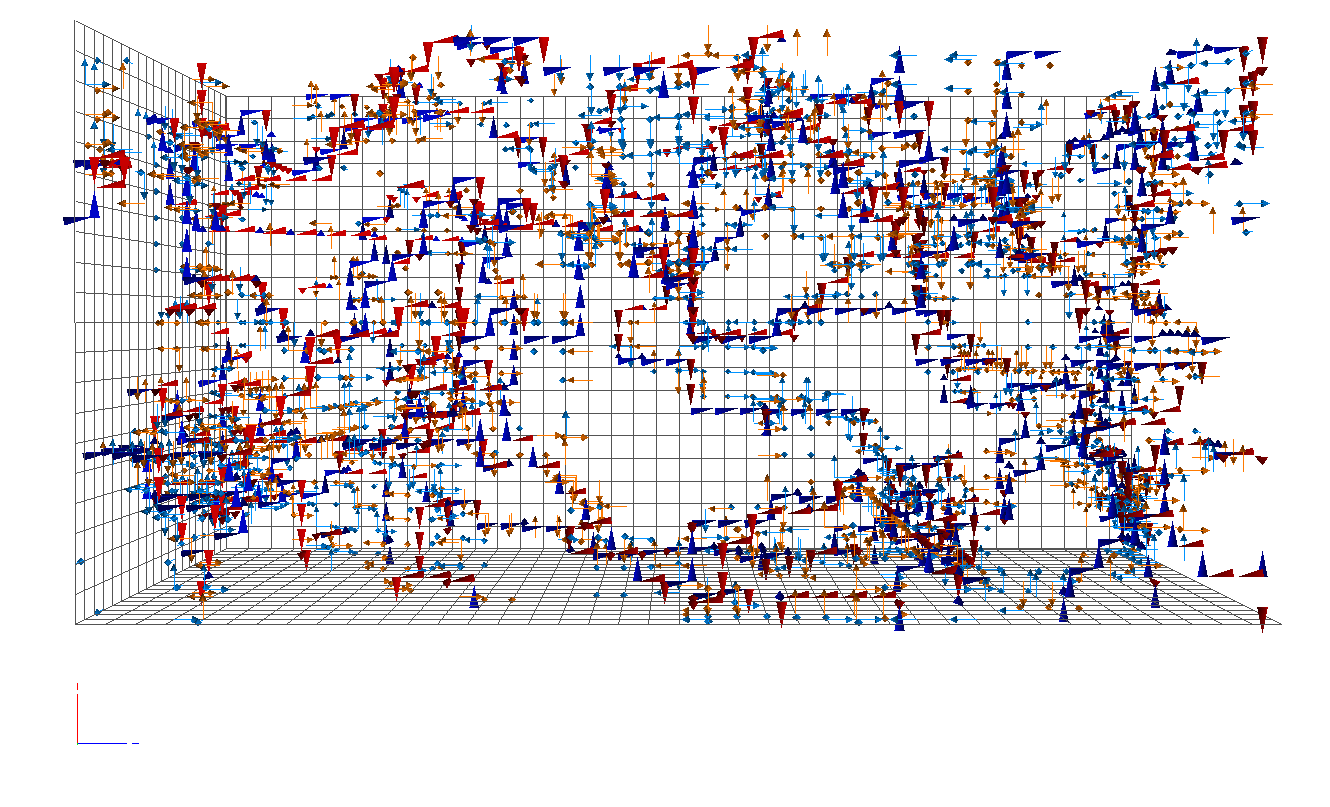
\includegraphics[width=\linewidth]{PlaqLink_CFG95_T01.png}
\caption{\label{fig:PlaqLinkT01}The $t=1$ slice with all space-oriented and time-oriented vortices plotted.}
\end{figure}
%
\begin{figure}
\centering
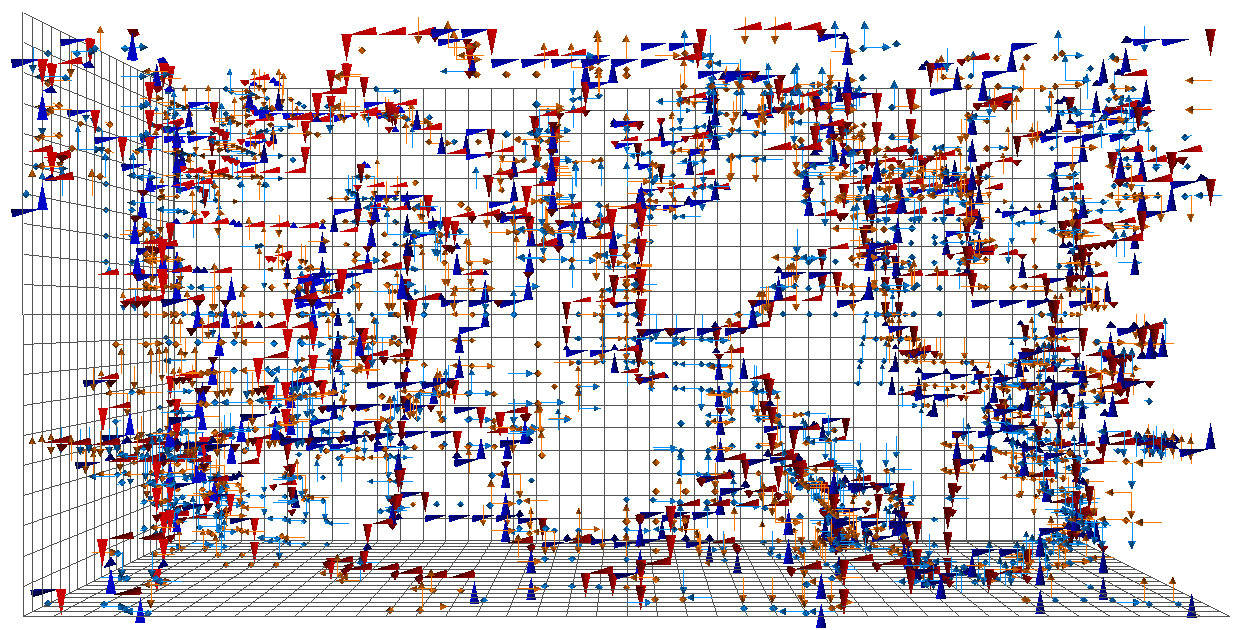
\includegraphics[width=\linewidth]{PlaqLink_CFG95_T02.png}
\caption{\label{fig:PlaqLinkT02}The $t=2$ slice with all space-oriented and time-oriented vortices plotted.}
\end{figure}
%

As we step through time, we expect to see the positively oriented vortices retain their colour but swap direction as they transition from being forwards in time to backwards in time, as shown in Fig.~\ref{fig:VortexArrows}. The time-oriented vortices act as predictors of vortex motion between slices. To see this, consider Fig.~\ref{fig:VortexMotion}. In Fig.~\ref{fig:VortexMotion1}, we observe a line of four $-1$ (red) space-oriented vortices with no time-oriented links associated with them, indicating that this line should remain fixed as we step through time. Alternatively, towards the top of the red line we observe a branching point with two associated $-1$ time-oriented arrows, indicating that this branching point should move in the direction of the time-oriented vortices. Observing the same region at $t=2$ in Fig.~\ref{fig:VortexMotion2}, we see that this is precisely what occurs. The vortex line has remained fixed, whereas the branching point has shifted one lattice spacing to the left, in accordance with the direction indicated by the time-oriented vortex.\\
%
\begin{figure}[htb!]
\centering
\begin{subfigure}[b]{0.45\textwidth}
\centering
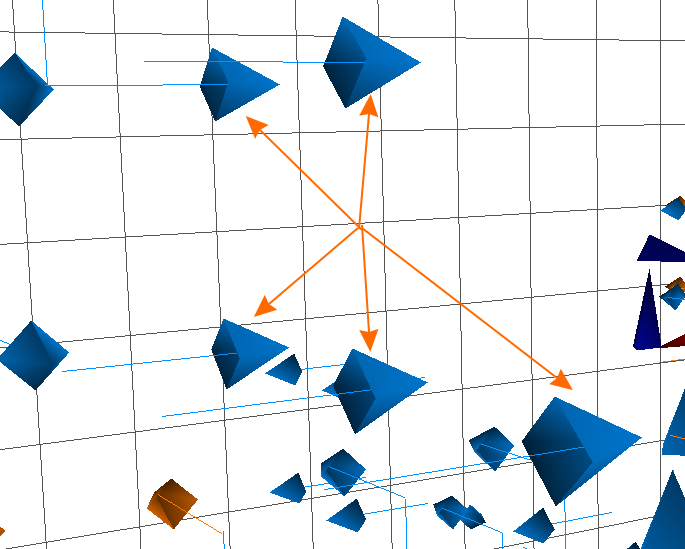
\includegraphics[height=0.2\textheight]{./plaqlinet1_forwardarrows.png}
\subcaption{\label{fig:VortexArrows1}$t=1$}
\end{subfigure}
\hfill
\begin{subfigure}[b]{0.45\textwidth}
\centering
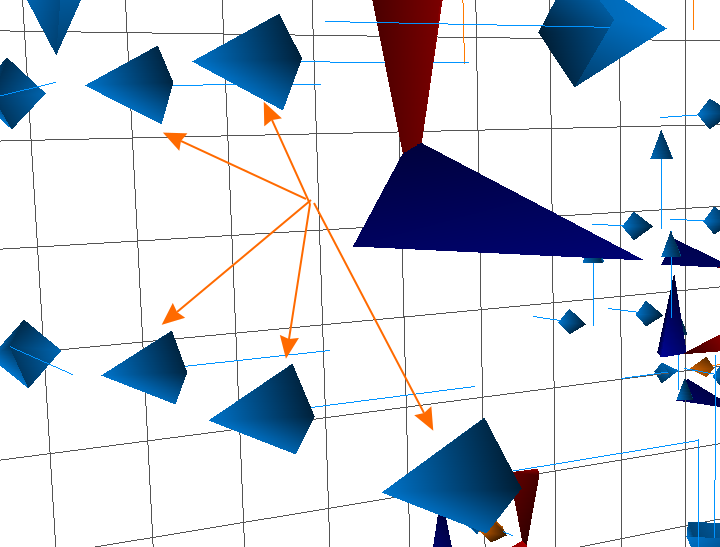
\includegraphics[height=0.2\textheight]{./plaqlinet2_backwardarrows.png}
\caption{\label{fig:VortexArrows2}$t=2$}
\end{subfigure}
\caption{\label{fig:VortexArrows}As we step through time we observe the time-oriented arrows change direction, however the phase (colour) of the vortex remains the same.}
\end{figure}
%
\begin{figure}
\centering
\begin{subfigure}[b]{0.45\textwidth}
\centering
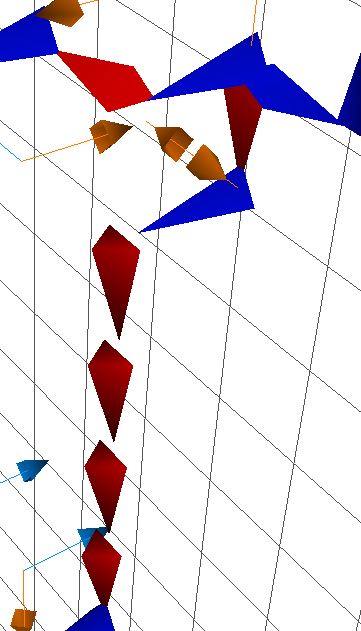
\includegraphics[height=0.4\textheight]{./plaqlinet1_line&monopole.png}
\subcaption{\label{fig:VortexMotion1}$t=1$}
\end{subfigure}
\hfill
\begin{subfigure}[b]{0.45\textwidth}
\centering
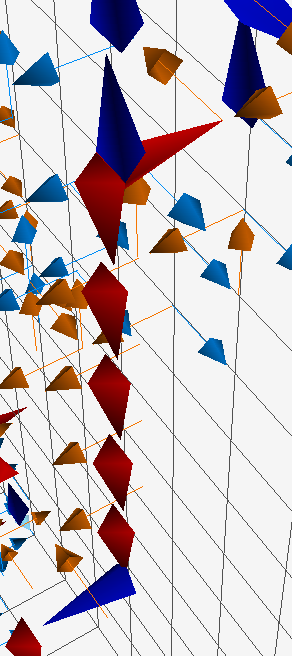
\includegraphics[height=0.4\textheight]{./plaqlinet2_line&monopole.png}
\caption{\label{fig:VortexMotion2}$t=2$}
\end{subfigure}
\caption{\label{fig:VortexMotion}An example of time-oriented vortices predicting the motion of the space-oriented vortices. We observe the $-1$ (red) vortex line with no associated time-oriented vortices remain stationary as we transition from $t=1$ to $t=2$.}
\end{figure}
%

Another example of time-oriented vortices predicting the motion of vortices is shown in Fig.~\ref{fig:VortexLineMotion}. Here we see in Fig.~\ref{fig:VortexLineMotion1} a line of three $+1$ space-oriented vortices each with an associated $-1$ time-oriented vortex below them. As we step to $t=2$ in Fig.~\ref{fig:VortexLineMotion2} we observe the time-oriented arrows change direction as expected, and the space-oriented vortex line shifts one lattice spacing down such that the time-oriented vortices are now above them.\\
%
\begin{figure}
\centering
\begin{subfigure}[b]{0.45\textwidth}
\centering
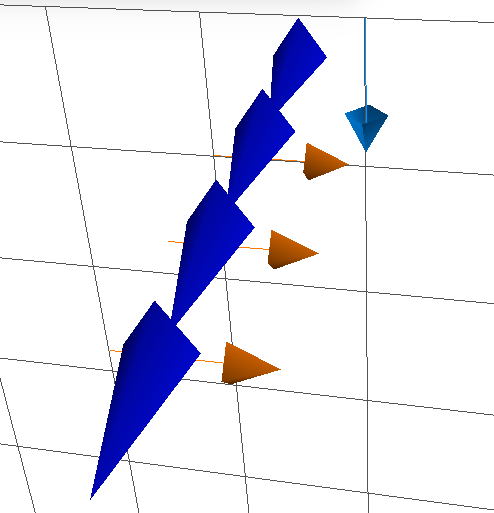
\includegraphics[height=0.3\textheight]{./plaqlinet1_SW8_line.png}
\subcaption{\label{fig:VortexLineMotion1}$t=1$}
\end{subfigure}
\hfill
\begin{subfigure}[b]{0.45\textwidth}
\centering
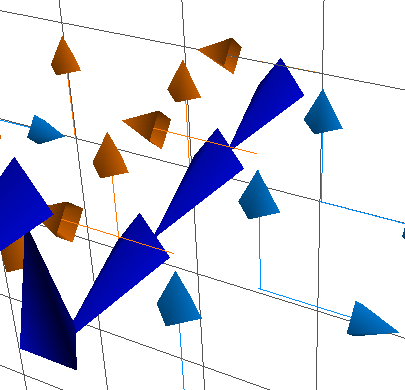
\includegraphics[height=0.3\textheight]{./plaqlinet2_SW8_line.png}
\subcaption{\label{fig:VortexLineMotion2}$t=2$}
\end{subfigure}
\caption{\label{fig:VortexLineMotion}A second example of time-oriented vortices predicting the motion of the space-oriented vortices. Here we see the $+1$ (blue) vortex line transition one lattice spacing down as we step from $t=1$ to $t=2$.}
\end{figure}
%

The cases presented in Fig.~\ref{fig:VortexMotion} and Fig.~\ref{fig:VortexLineMotion} are ideal, where the space-oriented vortex shifts only one lattice spacing between time slices. However, it is frequently the case where the space-oriented vortices shift multiple lattice spacings per time step. To see how this occurs diagrammatically, consider Fig.~\ref{fig:ComplexStructure}. The shaded red plaquettes indicate the location of a space-oriented vortex which would be plotted in the suppressed $\hat{x}$ direction. The red line demonstrates how the vortex line pierces between the two time slices. Within each slice we would observe the time-oriented links shown, however the space-oriented vortex appears to move three plaquettes in one time step. These multiple transitions make it harder to track the motion of vortices between time slices; nevertheless, the time-oriented vortices are a useful tool for understanding how centre vortices evolve with time. It is worth making clear that if a space-oriented vortex has no associated time-oriented vortices then it is guaranteed to remain stationary. In this respect, the lack of time-oriented vortices is a clear and valuable indicator of vortex behaviour.
%
\begin{figure}
\centering
\def\angThe{30}
\def\angPhi{0}

\tdplotsetmaincoords{\angThe}{\angPhi}
\scalebox{0.6}{\begin{tikzpicture}[tdplot_main_coords]

% Axes
\tkzDefPoint(-5,2){ax}
\tkzDefShiftPoint[ax](2,0){axR}
\tkzDefShiftPoint[ax](0,2){axT}
\tkzDefShiftPoint[ax](1.2,1.6){axB}

\begin{scope}[very thick,decoration={
    markings,
    mark=at position 0.5 with {\arrow[scale=2]{stealth}}}
    ] 
% Vortex line part 1
	\draw[line width=2,color=red,postaction={decorate}] (-3.6, -2.15) -- (-0.25,0);
	
% Bottom left red plaquette 
	\path[fill=red,opacity=0.3] (1,-1.5)--(3.5,1.5)--(-1.5,1.5)--(-4,-1.5)--cycle;
	\draw[line width=6,color=orange,-{Latex[length=6mm]}](1,-1.5)--(3.5,1.5);	
	
	\draw[line width=0.75,postaction={decorate}] (1,-1.5)-- node{} (3.5,1.5)node(g){};
	\draw[line width=0.75,postaction={decorate}](3.5,1.5)-- node{} (-1.5,1.5);
		
	\draw[pattern=north west lines, pattern color=orange](3.5,6.5) -- (1,3.5) -- (1,-1.5) -- (3.5,1.5) -- cycle;
	
	% Vortex line part 2
	\draw[line width=2,color=red,postaction={decorate}] (-0.25,0) -- (12.25,8);	
	
	\draw[line width=0.75,postaction={decorate}](-1.5,1.5)--node{}(-4,-1.5);  
	\draw[line width=0.75,postaction={decorate}] (-4,-1.5) --node{}(1,-1.5)node(f){};

% Top left empty plaquette
	\draw[line width=0.75](-1.5,1.5) -- (1,4.5);
	\draw[line width=0.75](1,4.5) -- (6,4.5);
	\draw[line width=0.75](3.5,1.5) -- (6,4.5);
	
% Bottom of dotted cubes
	\draw[line width=6,color=orange,-{Latex[length=6mm]}](8.5,1.5) -- (11,4.5);
	\draw[line width=6,color=cyan,-{Latex[length=6mm]}](3.5,1.5) -- (8.5,1.5);
	\draw[line width=0.75,dashed] (1,-1.5) -- (6,-1.5);
	\draw[line width=0.75,dashed] (3.5,1.5) -- (8.5,1.5);
	\draw[line width=0.75,dashed] (6,4.5) -- (11,4.5);
	
	\draw[line width=0.75,dashed] (6,-1.5) -- (8.5,1.5);
	\draw[line width=0.75,dashed] (8.5,1.5) -- (11,4.5);
	
% Left side of dotted cubes
	\draw[line width=6,color=orange,-{Latex[length=6mm]}](3.5,6.5) -- (1,3.5);
	
	\draw[line width=0.75,dashed] (1,-1.5) -- (1,3.5);
	\draw[line width=0.75,dashed] (3.5,1.5) -- (3.5,6.5);
	\draw[line width=0.75,dashed] (6,4.5) -- (6,9.5);
	
	\draw[line width=0.75,dashed] (1,3.5) -- (3.5,6.5);
	\draw[line width=0.75,dashed] (3.5,6.5) -- (6,9.5);
	
% Top of dotted cubes
	\draw[line width=6,color=orange,-{Latex[length=6mm]}](11,9.5) -- (8.5,6.5);	
	\draw[line width=6,color=cyan,-{Latex[length=6mm]}](8.5,6.5) -- (3.5,6.5);
	\draw[pattern=north west lines, pattern color=cyan] (8.5,6.5) -- (3.5,6.5) -- (3.5,1.5) -- (8.5,1.5) -- cycle;
	
	\draw[line width=0.75,dashed] (1,3.5) -- (6,3.5);
	\draw[line width=0.75,dashed] (3.5,6.5) -- (8.5,6.5);
	\draw[line width=0.75,dashed] (6,9.5) -- (11,9.5);
	
	\draw[line width=0.75,dashed] (6,3.5)-- (8.5,6.5);
	\draw[line width=0.75,dashed] (8.5,6.5) -- (11,9.5);
	
% Right side of dotted cubes
	\draw[pattern=north west lines, pattern color=orange] (11,9.5) -- (8.5,6.5) --  (8.5,1.5) -- (11,4.5) -- cycle;
	
	\draw[line width=0.75,dashed] (6,3.5) -- (6,-1.5);
	\draw[line width=0.75,dashed] (8.5,6.5) -- (8.5,1.5);
	\draw[line width=0.75,dashed] (11,9.5) -- (11,4.5);
	
% Bottom right empty plaquette
	\draw[line width=0.75] (6,3.5) -- (11,3.5);
	\draw[line width=0.75] (11,3.5) -- (13.5,6.5);
	
% Top right red plaquette
	\path[fill=red,opacity=0.3] (8.5,6.5)--(13.5,6.5)--(16,9.5)--(11,9.5)--cycle;
	\draw[line width=0.75,postaction={decorate}] (8.5,6.5) -- (13.5,6.5);
	\draw[line width=0.75,postaction={decorate}] (13.5,6.5) -- (16,9.5);
	\draw[line width=0.75,postaction={decorate}] (16,9.5) -- (11,9.5);
	
% Vortex line part 3
	\draw[line width=2,color=red,postaction={decorate}] (12.25,8) -- (15.6,10.15);

% t labels
	\draw[line width=1,loosely dotted] (6,-1.5) -- (14,-1.5)node[right]{$\resizebox{1.5cm}{!}{t=1}$};
	\draw[line width=1,loosely dotted] (11,3.5) -- (14,3.5)node[right]{$\resizebox{1.5cm}{!}{t=2}$};
	
% Draw Axes
\tkzDrawSegments[thick,->, >=stealth](ax,axR)
\tkzDrawSegments[thick,->, >=stealth](ax,axT)
\tkzDrawSegments[thick,->, >=stealth](ax,axB)
\tkzLabelPoint[right](axR){$\resizebox{0.3cm}{!}{y}$}
\tkzLabelPoint[above](axT){$\resizebox{0.3cm}{!}{t}$}
\tkzLabelPoint[above](axB){$\resizebox{0.3cm}{!}{z}$}
  \end{scope}
\end{tikzpicture}}

\caption{\label{fig:ComplexStructure}A demonstration of how space-oriented vortices can transition multiple lattice spacings in a single time step.}
\end{figure}

\section{Topological Charge}\label{sec:TopChargeVis}
We now wish to observe the relationship between vortices and topological charge. As stated in Sec.~\ref{sec:TopQ}, the topological charge density is given by
%
\begin{equation}
q ( x ) = \frac { 1 } { 32 \pi ^ { 2 } } \, \epsilon _ { \mu \nu \rho \sigma } \, \Tr\left( F _ { \mu \nu }( x ) \, F _ { \rho \sigma }(x) \right) \, .
\end{equation}
%
Given the presence of the antisymmetric tensor, it is clear that for there to be non-trivial topological charge present on the projected vortex configurations, we require that the tangent vectors of the vortex surface span all four dimensions. This condition is met at \textit{singular points}, which can be broken into three categories~\cite{Engelhardt:2010ft,Engelhardt:2000wc}
\begin{enumerate}
\item Intersection points.
\item Touching points.
\item Writhing points.
\end{enumerate}
The contribution to the topological charge from these singular points is discussed in detail in Refs.~\cite{Bruckmann:2003yd,Engelhardt:2010ft,Engelhardt:2000wc,Engelhardt:1999xw}. In our visualisations, these singular points appear as a space-oriented vortex running parallel to a time-oriented vortex, as shown in Fig.~\ref{fig:SingularPoint}.\\
%
\begin{figure}[htb!]
\centering
\begin{tikzpicture}[scale=0.9]
\begin{scope}[very thick,decoration={
    markings,
    mark=at position 0.5 with {\arrow[scale=2]{stealth}}}
    ] 

  % orange line first to make it look transparent
  \draw[line width=6,color=orange,-{Latex[length=6mm]}](-4.0,-1.5)--(-4.0,4.0);

  % bottom right to top right                    x,y start of line    label  x,y end
  \draw[line width=1.0,postaction={decorate}](1.5,-1.5)--node[right]{} (3.25,1.5)node(g){};
  % top right to top left
  \draw[line width=1.0,postaction={decorate}](3.25,1.5)--node[above]{} (-1.5,1.5);
  % top left to bottom left
  \draw[line width=1.0,postaction={decorate}](-1.5,1.5)--node[left]{} (-4,-1.5);

  % Jet triangle
  % bottom left	
  \draw (-0.3,-2) node(a){}
  -- (0.1,-2) node(b){}   % bottom right
  -- (-0.1,2) node(c){}   % top
  -- cycle;               % complete
  \fill[blue] (a.center) -- (b.center) -- (c.center);
  
  % bottom left to bottom right
  \draw[line width=1.0,postaction={decorate}](-4,-1.5)--node[above]{}(1.5,-1.5)node(f){};
  
  % z direction  
  \draw[line width=1.0,postaction={decorate}]( 1.5,-1.5)--node[right]{} (1.5,4.0);    % width  3.25-(-1.5) = 4.75
  \draw[line width=1.0,postaction={decorate}]( 1.5, 4.0)--node[above]{}(-4.0,4.0);    % height 6.25-1.5    = 4.75
  \draw[line width=1.0,postaction={decorate}](-4.0, 4.0)--node[left]{}(-4.0,-1.5);

  % Coordinate axes       arrow head          x,y start -- x,y finish [position] label
  \draw[line width=1.0,-{Latex[length=2mm]}](3,-1.5)--(4,-1.5)node[right]{\large $x$};
  \draw[line width=1.0,-{Latex[length=2mm]}](3,-1.5)--(3.4,-0.7)node[right]{\large $y$};
  \draw[line width=1.0,-{Latex[length=2mm]}](3,-1.5)--(3,-0.5)node[above]{\large $z$};
  \end{scope}
\end{tikzpicture}
\caption{\label{fig:SingularPoint} The signature of a singular point, in which the vortex surface spans all four directions. The colour and orientation of the vortices is irrelevant, so long as they are parallel.}
\end{figure}
%

We calculate the topological charge via the method outlined in Sec.~\ref{sec:TopQ} on a lattice configuration after eight sweeps of cooling. This cooling is necessary to remove short-range fluctuations, but is a sufficiently low number of sweeps so as to minimally perturb the configuration. We plot regions of positive topological charge in blue, and regions of negative topological charge in red, with a colour gradient to indicate the magnitude. Only topological charge of sufficient magnitude is plotted to better emphasise regions of significant topological charge. Overlaying the topological charge visualisation onto Figs.~\ref{fig:PlaqLinkT01}, \ref{fig:PlaqLinkT02}, we obtain Figs.~\ref{fig:PlaqLinkQT01}, \ref{fig:PlaqLinkQT02}. By studying the regions of high topological charge, we note that we can indeed observe their relationship with singular points, as shown in Fig.~\ref{fig:SingularPointVis}.\\
%
\begin{figure}
\centering
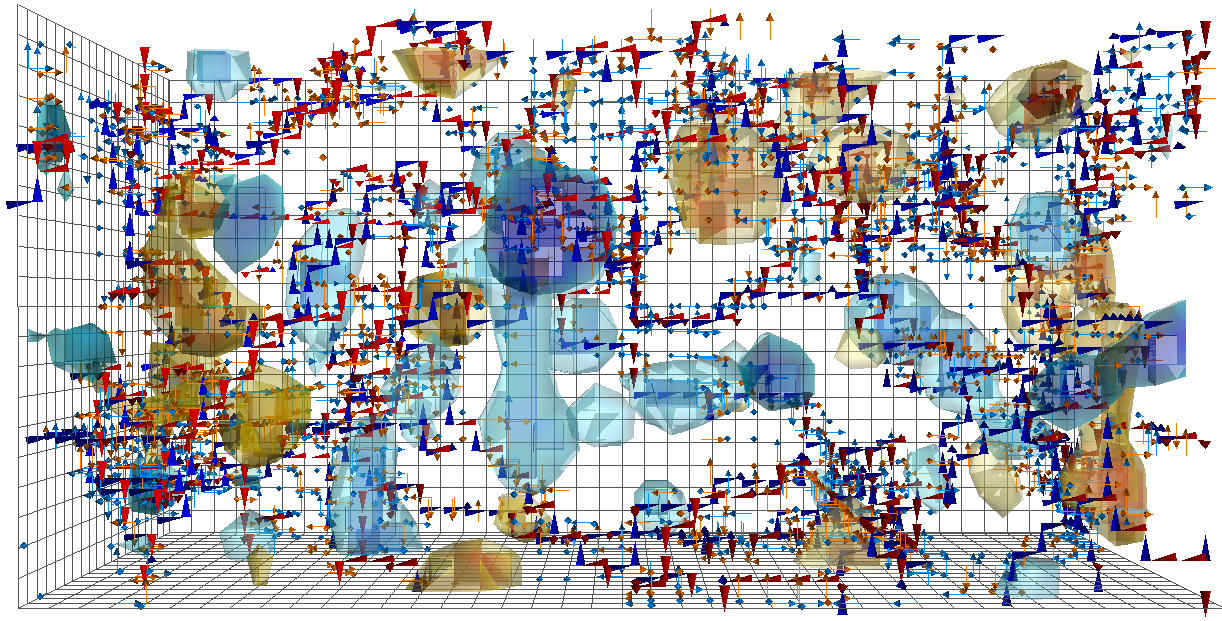
\includegraphics[width=\linewidth]{./PlaqLinkTopQ_CFG95_T01.png}
\caption{\label{fig:PlaqLinkQT01}Topological charge density overlaying the $t=1$ slice.}
\end{figure}
%
\begin{figure}
\centering
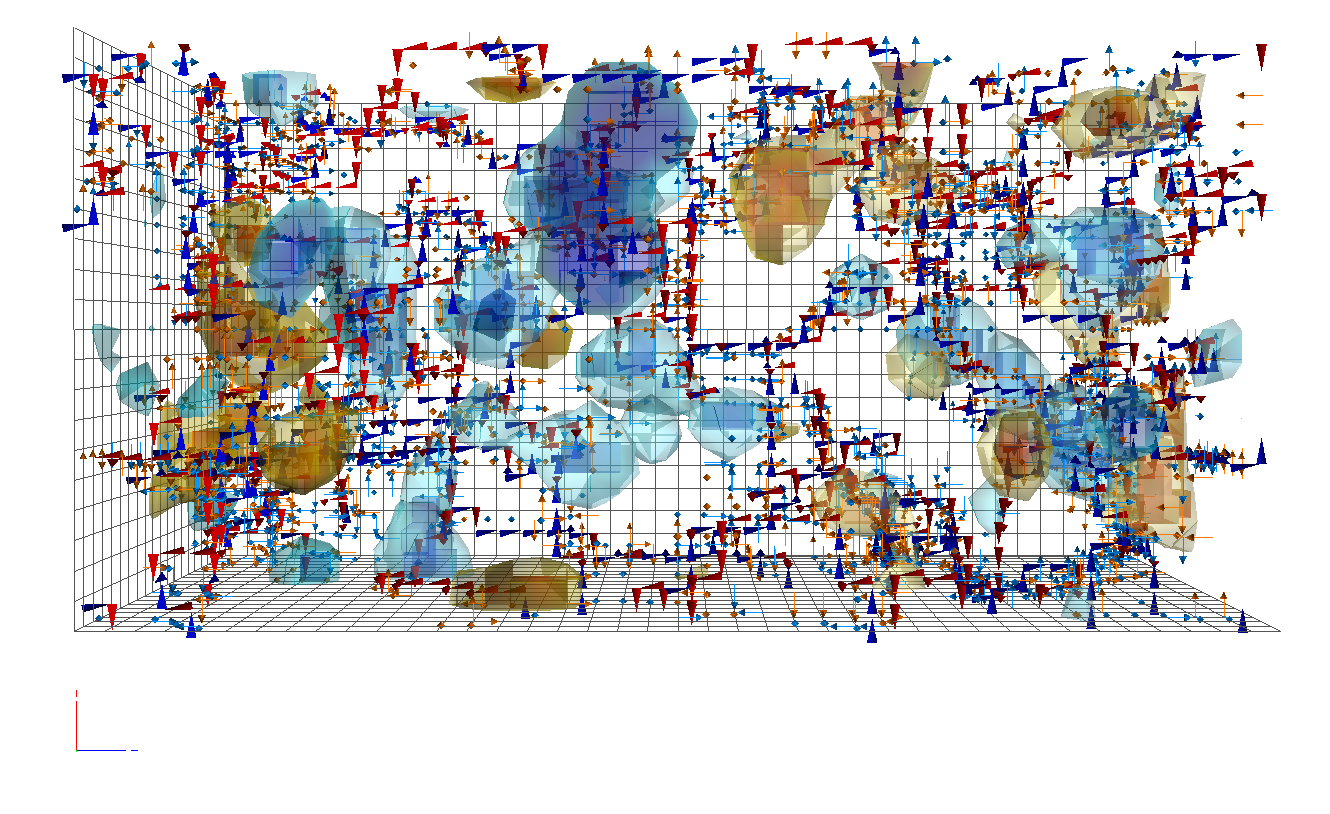
\includegraphics[width=\linewidth]{./PlaqLinkTopQ_CFG95_T02.png}
\caption{\label{fig:PlaqLinkQT02}Topological charge density overlaying the $t=2$ slice.}
\end{figure}
%
\begin{figure}[htb!]
\centering
\begin{subfigure}[b]{0.45\textwidth}
\centering
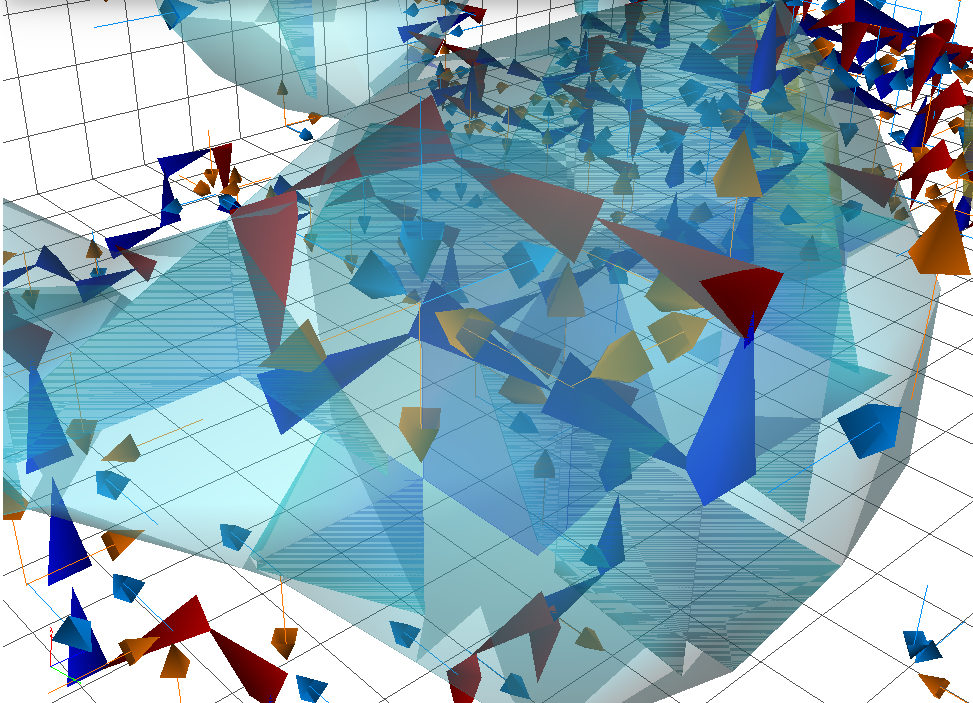
\includegraphics[height=0.2\textheight]{./PlaqLinkQt2_SingularCollection.png}
\end{subfigure}
\hfill
\begin{subfigure}[b]{0.5\textwidth}
\centering
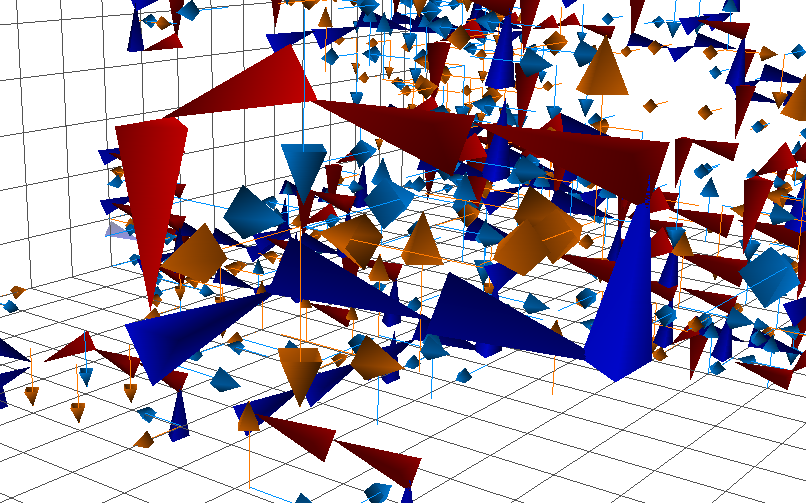
\includegraphics[height=0.2\textheight]{./PlaqLinkt2_SingularCollection.png}
\end{subfigure}
\caption{\label{fig:SingularPointVis}A collection of singular points shown with (left) and without (right) topological charge overlaid.}
\end{figure}
%

To quantify the correlation between vortex locations and topological charge, we use the following measure
%
\begin{equation}
C = V\frac{\sum_x |q(x)|\,L(x)}{\sum_x |q(x)|\,\sum_x L(x)}\, ,
\end{equation}
%
where $V$ is the lattice volume, and
%
\begin{equation}
L(x) = 
\begin{cases}
1\, , & \text{Vortex associated with any plaquette touching $x$}\\
0\, , & \text{No vortex associated with any plaquette touching $x$}\, .
\end{cases}
\end{equation}
%
In the case of no correlation, $C=1$. If there is correlation or anti-correlation, then $C>1$ or $C<1$ respectively. The value of $C$ for our configurations is shown in Fig.~\ref{fig:Correlation}, with an average over all 100 configurations of $\bar{C} = 1.46$. This indicates a correlation between vortex locations and regions of high topological charge. Further work to investigate the precise nature of this correlation and its relationship to singular points is planned.\\
%
\begin{figure}[htb!]
\centering
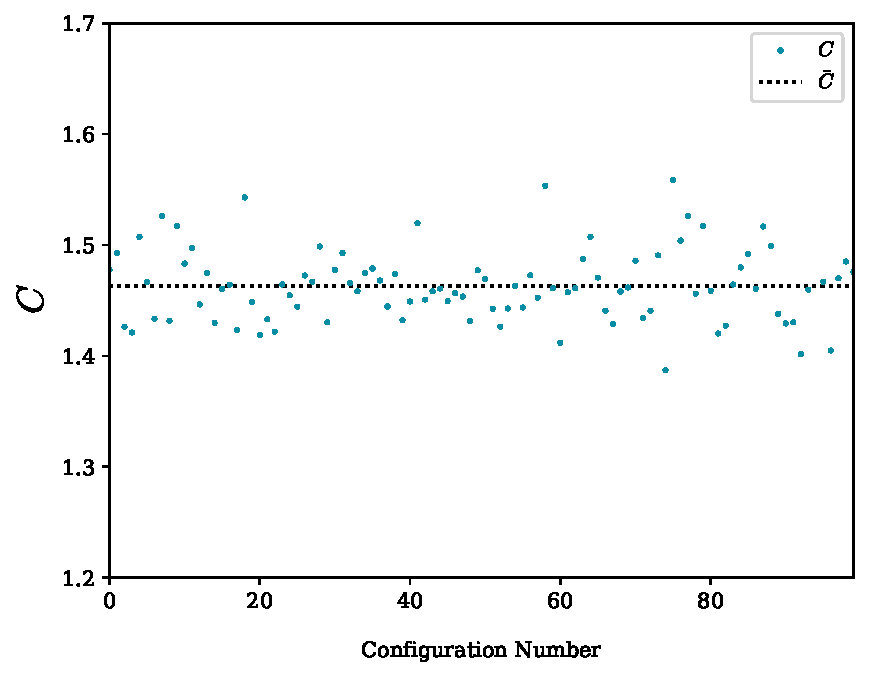
\includegraphics[width=0.8\linewidth]{./Correlation.pdf}
\caption{\label{fig:Correlation} The correlation measure for each configuration is shown. The dashed line indicates the average value across all 100 configurations, with the one standard deviation region shown in green.}
\end{figure}
%
\begin{figure}
\centering
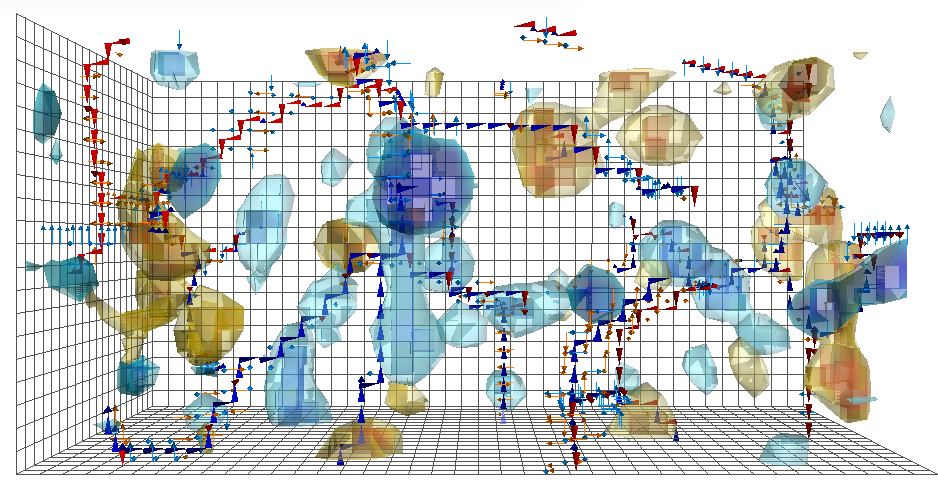
\includegraphics[width=\linewidth]{./PlaqLinkTopQ_CFG95_T01_8SW.png}
\caption{\label{fig:PlaqLinkTopQ_SW8}The vortex structure and topological charge after eight sweeps of cooling, for $t=1$.}
\end{figure}
%

Finally, it is also interesting to study the vortex structure of the lattice after cooling. After eight sweeps of cooling, we obtain Fig.~\ref{fig:PlaqLinkTopQ_SW8}. We clearly see that the complexity of the vortex structure has been greatly reduced, however the regions associated with topological charge have been less affected by the smoothing process. We can see this by recalculating the topological charge, shown in Fig.~\ref{fig:Correlation_sw07}. The average correlation has increased to a new average of $\bar{C}=1.76$, indicating that the residual vortices show a stronger correlation to the regions of high topological charge than those on the un-cooled configurations. This further supports the previously mentioned notion that cooling serves to isolate `genuine' topological objects and filter out those arising from fluctuations during the monte-carlo lattice generation process.
%

\begin{figure}
\centering
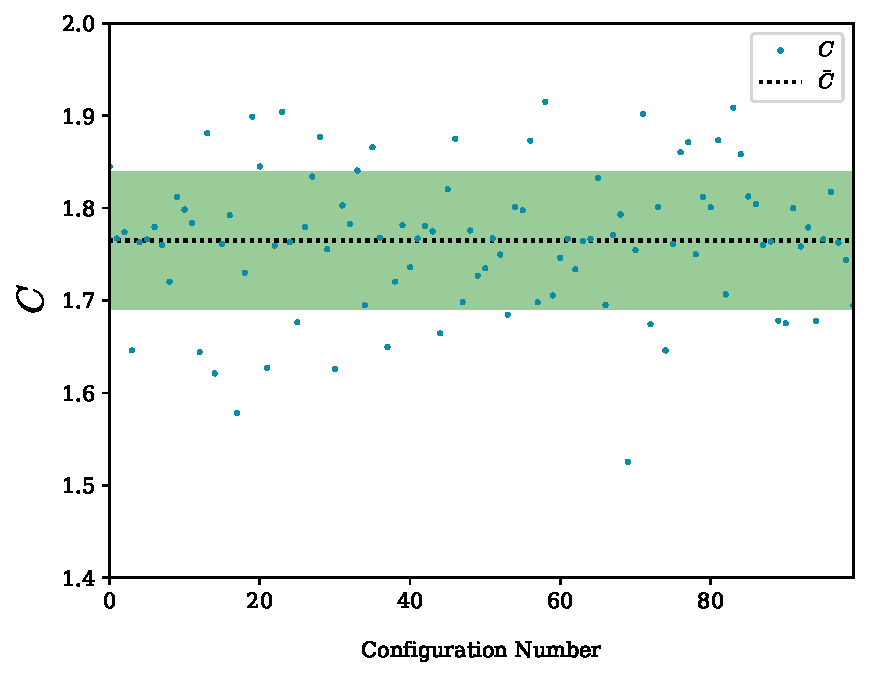
\includegraphics[width=0.8\linewidth]{./Correlation_sw07.pdf}
\caption{\label{fig:Correlation_sw07}The correlation measure for each configuration after eight sweeps of cooling is shown. The dashed line indicates the average value across all 100 configurations, with the one standard deviation region shown in green.}
\end{figure}

\section{Summary}
In this chapter we have presented a new way to visualise the four-dimensional structure of centre vortices on the lattice through the use of 3D visualisation techniques. These visualisations give new insight into the geometry and time-evolution of vortices, as well as revealing a direct connection to topological charge. The work presented here is preliminary, and in future it would be valuable to improve the ability to identify branching/monopole points and singular points such that they may be studied in a more quantitative way. Developing techniques to categorise the nature of singular points to further elucidate their connection to topological charge would also be another worthwhile avenue to pursue. From this work, it is clear that visualisations of centre vortices provide valuable information about the structure of the QCD vacuum that is otherwise not apparent through purely numerical results, and that visualisations elegantly complement more traditional calculation techniques.
